\documentclass{beamer}

%%%% Packages
\usepackage{amsmath, amsthm, amssymb}
\usepackage[english]{babel}
\usepackage{algpseudocode}      % algorithmic environment
\usepackage{array}              % for >{} in table column
                                % specification
\usepackage{color}              % for color definition
\usepackage{colortbl}
\usepackage{graphicx}
\usepackage{multirow}           % for multirow
\usepackage{multicol}           % for multiple columns
\usepackage{tabularx}           % for centering in table
\usepackage{tikz}               % for drawing diagrams
\usetikzlibrary{arrows}
\usetikzlibrary{positioning}

%%%% Macros and Definitions
\definecolor{firebrick4}{RGB}{139,026,026}
\definecolor{gray57}{RGB}{145,145,145}
\definecolor{gray71}{RGB}{181,181,181}
\definecolor{gray84}{RGB}{212,212,212}
\definecolor{lightcyan4}{RGB}{122,139,139}
\definecolor{dodgerblue4}{RGB}{16,78,139}
\definecolor{dodgerblue3}{RGB}{24,116,205}
\definecolor{lightcyan4}{RGB}{122,139,139}

\setcounter{tocdepth}{1}

\newlength{\picwidth}
\setlength{\picwidth}{2.5cm}
\newlength{\picheight}
\setlength{\picheight}{2cm}
\newlength{\oosixthClmnWidth}
\setlength{\oosixthClmnWidth}{0.05\textwidth}

\newlength{\firstcolumnwidth}
\setlength{\firstcolumnwidth}{0.25\textwidth}
\newlength{\mycolumnwidth}
\setlength{\mycolumnwidth}{0.13\textwidth}

\newcommand{\lexiconlimit}{Limitedness of machine-readable lexicons}
\newcommand{\genrespecifics}{Stylistic specifics of text genre}

\newcommand{\totaloov}{\% of OOV tokens}
\newcommand{\uniqoov}{\% of OOV types}

\newcommand{\totalHunspellDictToken}{45.87}
\newcommand{\totalHunspellDictType}{54.62}
\newcommand{\totalTTaggerDictToken}{40.46}
\newcommand{\totalTTaggerDictType}{43.36}

\newcommand{\totalHunspellStyleToken}{41.65}
\newcommand{\totalHunspellStyleType}{33.64}
\newcommand{\totalTTaggerStyleToken}{48.02}
\newcommand{\totalTTaggerStyleType}{44.59}

\newcommand{\totalHunspellSpellToken}{11.87}
\newcommand{\totalHunspellSpellType}{10.75}
\newcommand{\totalTTaggerSpellToken}{9.09}
\newcommand{\totalTTaggerSpellType}{8.23}

\newcommand{\normquestions}[4]{
  Questions regarding text normalization:
  \begin{itemize}
    \item How relevant is text normalization for German tweets? \textit{#1}
    \item What should be normalized? \textit{#2}
    \item How should we normalize? \textit{#3}
    \item How can we measure the quality of text normalization? \textit{#4}
  \end{itemize}
}

%%%% Presentation Setup
\mode<presentation>
{
  \usetheme{Ilmenau}
  \usecolortheme{beaver}
  \usefonttheme[onlylarge]{structuresmallcapsserif}
}
\setbeamercolor{title}{fg=dodgerblue4}
\setbeamercolor{frametitle}{fg=dodgerblue4}
\setbeamercolor*{palette secondary}{fg=dodgerblue4,bg=gray84}
\setbeamercolor*{palette tertiary}{fg=white,bg=dodgerblue4}
\setbeamercolor*{item}{fg=dodgerblue4}

\setbeamerfont{author}{size=\scriptsize}
\setbeamerfont{institute}{size=\scriptsize}
\setbeamerfont{date}{size=\tiny}
\setbeamerfont{normal text}{size=\scriptsize}

\beamertemplatenavigationsymbolsempty

%%%% Title
\title[Sentiment Analysis]{Fine-grained Sentiment Analysis on German Twitter}
\author[Sidorenko]{Wladimir Sidorenko\\ \texttt{uladzimir.sidarenka{@}uni-potsdam.de}}
\institute[Uni Potsdam]{University of Potsdam}
\date{\today}

\pgfdeclareimage[interpolate=true,height=2.5cm]{logo}{img/uni_potsdam_logo.png}
\titlegraphic{\pgfuseimage{logo}}

%%%% Document
\begin{document}
%%%%%%%%%%%%%%%%%%%%%%%%%%%%%%%%%%%%%%%%%%%%%%%%%%%%%%%%%%%%%%%%%%
%%% Title Page
\begin{frame}{}
  \titlepage
\end{frame}

%%%%%%%%%%%%%%%%%%%%%%%%%%%%%%%%%%%%%%%%%%%%%%%%%%%%%%%%%%%%%%%%%%
%%% Table of Contents
\begin{frame}{Table of Contents}
  \tableofcontents
\end{frame}

%%%%%%%%%%%%%%%%%%%%%%%%%%%%%%%%%%%%%%%%%%%%%%%%%%%%%%%%%%%%%%%%%%
%%% Text Normalization
\section{Text Normalization}

\begin{frame}{}
  Twitter messages are different from newspaper articles and other
  types of texts.
  \begin{example}
    ohja -- \#sadbrasilian RT @CorneliusBaier: Die beste \#BRAGER -
    Geschichte \"uberhaupt:
    http://mashable.com/2014/07/09/brazil-germany-world-cup-sweet-moment/...
  \end{example}

  \begin{example}
    Eins zu 4500, auf diese Quote bezifferte US-Statistikexperte Nate
    Silver die M\"oglichkeit, dass Deutschland sieben Tore
    schie\ss{}t.  \end{example}
\end{frame}

\begin{frame}{}
  Questions regarding Twitter specifics:
  \begin{itemize}
    \item What are the differences between tweets and standard language texts?
    \item Do we need to do something against these differences?  And
      what should we do, if yes?
  \end{itemize}
\end{frame}

\begin{frame}{}
  Differences between tweets and other text genres are primarily
  caused by a high rate of unknown (out-of-vocabulary) words, and
  these words really form a problem for existing NLP applications.
  \begin{example}
    \alert{Leg\_NN} den\_ART Karl\_NE weg\_PTKVZ ,\_\$,
    \alert{denn\_KON} kannste\_VVFIN immer\_ADV noch\_ADV hauen\_VVINF
    ,\_\$, der\_ART heutige\_ADJA \alert{@Tatort\_NN} ist\_VAFIN
    mal\_ADV wieder\_ADV richtig\_ADJD gut\_ADJD :\_: \alert{-D\_ADJA}
  \end{example}
\end{frame}

\begin{frame}{}
  What can we do against unknown words?  Possible solutions are:
  \begin{itemize}
    \item<+-> adjust the tools (domain adaptation);
    \item<+->  adjust the text (text normalization).
  \end{itemize}
\end{frame}

\begin{frame}{}
  \normquestions{}{}{}{}
\end{frame}

\begin{frame}{}
  \textbf{10,000} randomly selected tweets from a corpus of 24,179,871 Twitter
  messages that were gathered in April 2013.  After sentence splitting and
  tokenization we got a list of \textbf{129,146} tokens (\textbf{32,538} token
  types).  These tokens were successively processed with open source tools
  \texttt{hunspell} and \texttt{TreeTagger}.
\end{frame}

\begin{frame}{Rate of OOV Tokens}
  \footnotesize From the previously obtained token list, 26,018 tokens were
  considered as OOV by \texttt{hunspell}, and 28,389 were regarded as OOV by
  \texttt{TreeTagger}.
  \begin{table}
    \caption{OOV rate in analyzed tweets}
    \begin{tabular}{p{\firstcolumnwidth}*{4}{>{\centering\arraybackslash}p{\mycolumnwidth}}}
      \hline\noalign{\smallskip}
      \multirow{2}{*}{} & %
      \multicolumn{2}{c}{\texttt{hunspell}} & %
      \multicolumn{2}{c}{\texttt{TreeTagger}}\\
      & \totaloov{} & \uniqoov{} & \totaloov{} & \uniqoov{}\\
      \noalign{\smallskip} \hline
      OOV rate & 20.15 & 46.96 & 21.98 & 58.24\\
      \noalign{\smallskip} \hline
    \end{tabular}
  \end{table}
\end{frame}

\begin{frame}{Classes of OOV-Tokens}
  In which classes can OOV-tokens be divided?\pause
  \begin{itemize}
    \item<+-> \lexiconlimit;
    \item<+-> \genrespecifics;
    \item<+-> Sloppiness of user input.
  \end{itemize}
\end{frame}

\begin{frame}{}
  In order to measure how OOV-tokens were distributed among these
  classes, we selected and analyzed all OOV-tokens with frequency
  higher than 1 and also took 1,000 randomly selected hapax legomena.
\end{frame}

\begin{frame}{}
  \begin{table}
    \footnotesize
    \caption{Distribution of OOV-tokens among three major classes}
    \begin{tabular}{>{\scriptsize}p{\firstcolumnwidth}*{4}{>{\centering\arraybackslash}p{\mycolumnwidth}}}
      \hline\noalign{\smallskip}
      \multirow{2}{*}{OOV class} & %
      \multicolumn{2}{c}{\texttt{hunspell}} & %
      \multicolumn{2}{c}{\texttt{TreeTagger}}\\
      & \totaloov{} & \uniqoov{} & \totaloov{} & \uniqoov{}\\
      \noalign{\smallskip} \hline
      Limitedness of lexicons & \totalHunspellDictToken & %
      \totalHunspellDictType & %
      \totalTTaggerDictToken & \totalTTaggerDictType\\
      Stylistic specifics of text genre & \totalHunspellStyleToken & %
      \totalHunspellStyleType & %
      \totalTTaggerStyleToken %
      & \totalTTaggerStyleType\\
      Deviating spelling & \totalHunspellSpellToken & %
      \totalHunspellSpellType & \totalTTaggerSpellToken & %
      \totalTTaggerSpellType\\
      \noalign{\smallskip} \hline
    \end{tabular}
  \end{table}
\end{frame}

\begin{frame}{}
  \scriptsize
  \begin{table}
    \caption{\scriptsize Distribution of OOV-tokens in the class
      ``\lexiconlimit''} \centering
    \begin{tabular}{p{\firstcolumnwidth}*{4}{>{\centering\arraybackslash}p{\mycolumnwidth}}}
      \hline\noalign{\smallskip}
      \multirow{2}{*}{OOV subclass} & %
      \multicolumn{2}{c}{\texttt{hunspell}} & %
      \multicolumn{2}{c}{\texttt{TreeTagger}}\\
      & \totaloov{} & \uniqoov{} & \totaloov{} & \uniqoov{}\\
      \noalign{\smallskip} \hline
      Common German words & 7.27 & 8.66 & 2.74 & 3.46\\
      Compounds & 1.27 & 2.65 & 2.5 & 4.54\\
      Abbreviations & 3.96 & 4.8 & 3.26 & 3.43\\
      Interjections & 5.99 & 4.6 & 5.56 & 4.27\\
      Person names & 4.77 & 6.49 & 2.31 & 3.46\\
      Geographical names & 1.53 & 2.6 & 1.16 & 1.87\\
      Company names & 2.28 & 2.87 & 4.34 & 3\\
      Product names & 2.16 & 2.65 & 2.45 & 3.22\\
      Neologisms & 1.37 & 1.35 & 3.32 & 2.38\\
      Loan words & 3.7 & 4.06 & 3.28 & 2.86\\
      Foreign words & 11.57 & 13.89 & 9.54 & 10.87\\\hline
      {\bfseries Total} & \totalHunspellDictToken & %
      \totalHunspellDictType & \totalTTaggerDictToken & %
      \totalTTaggerDictType\\
      \noalign{\smallskip} \hline
    \end{tabular}
  \end{table}
\end{frame}

\begin{frame}{}
  \scriptsize
  \begin{table}
    \caption{\footnotesize Distribution of OOV-tokens in the class
      ``\genrespecifics{}''} \centering
    \begin{tabular}{p{\firstcolumnwidth}*{4}{>{\centering\arraybackslash}p{\mycolumnwidth}}}
      \hline\noalign{\smallskip}
      \multirow{2}{*}{OOV-Unterklasse} & %
      \multicolumn{2}{c}{\texttt{hunspell}} & %
      \multicolumn{2}{c}{\texttt{TreeTagger}}\\
      & \totaloov{} & \uniqoov{} & \totaloov{} & \uniqoov{}\\
      \noalign{\smallskip} \hline
      @-mentions & 13.12 & 20.49 & 16.14 & 21.84\\
      hashtags & 7.41 & 6.26 & 13.02 & 10.56\\
      hyperlinks & 2.45 & 0.4 & 4.88 & 6.05\\
      emoticons & 2.01 & 0.74 & 6.86 & 1.2\\
      slang words & 16.66 & 5.75 & 7.12 & 4.94\\\hline
      {\bfseries Total} & \totalHunspellStyleToken & %
      \totalHunspellStyleType & \totalTTaggerStyleToken & %
      \totalTTaggerStyleType\\
      \noalign{\smallskip} \hline
    \end{tabular}
  \end{table}
\end{frame}

\begin{frame}{}
  \footnotesize
  \begin{table}
    \caption{\footnotesize Intended (colloquial) vs. unintended (erroneous)
      ``spelling deviations''} \centering
    \begin{tabular}{>{\scriptsize}p{\firstcolumnwidth}*{4}{>{\centering\arraybackslash}p{\mycolumnwidth}}}
      \hline\noalign{\smallskip}
      \multirow{2}{*}{OOV-subclass} & %
      \multicolumn{2}{c}{\texttt{hunspell}} & %
      \multicolumn{2}{c}{\texttt{TreeTagger}}\\
      & \totaloov{} & \uniqoov{} & \totaloov{} & \uniqoov{}\\
      \noalign{\smallskip} \hline
      Intended deviations, e.g. \textit{Tach}, \textit{nen} & 8.06 & 5.09 & 5.97 & 3.7\\
      Unintended deviations, e.g. \textit{michte}, \textit{Geschhen} & 3.81 & 5.66 & 3.12 & 4.54\\\hline
      {\bfseries Total} & \totalHunspellSpellToken & \totalHunspellSpellType & %
      \totalTTaggerSpellToken & \totalTTaggerSpellType\\
      \noalign{\smallskip} \hline
    \end{tabular}
  \end{table}
\end{frame}

\begin{frame}{}
  \footnotesize
  \begin{table}
    \caption{\footnotesize Distribution of OOV-tokens in the class ``Spelling
      deviations''} \centering
    \begin{tabular}{>{\scriptsize}p{\firstcolumnwidth}*{4}{>{\centering\arraybackslash}p{\mycolumnwidth}}}
      \hline\noalign{\smallskip}
      \multirow{2}{*}{OOV-subclass} & %
      \multicolumn{2}{c}{\texttt{hunspell}} & %
      \multicolumn{2}{c}{\texttt{TreeTagger}}\\
      & \totaloov{} & \uniqoov{} & \totaloov{} & \uniqoov{}\\
      \noalign{\smallskip} \hline
      Insertions & 1 & 1.66 & 0.79 & 1.08\\
      Deletions & 8.3 & 6.28 & 6.55 & 5.33\\
      Substitutions & 2.57 & 2.81 & 1.75 & 1.82\\\hline
      {\bfseries Total} & \totalHunspellSpellToken & %
      \totalHunspellSpellType & \totalTTaggerSpellToken & %
      \totalTTaggerSpellType\\
      \noalign{\smallskip} \hline
    \end{tabular}
  \end{table}
\end{frame}

\begin{frame}{}
  \begin{table}
    \footnotesize
    \caption{Distribution of OOV-tokens among three major classes}
    \begin{tabular}{>{\scriptsize}p{\firstcolumnwidth}*{4}{>{\centering\arraybackslash}p{\mycolumnwidth}}}
      \hline\noalign{\smallskip}
      \multirow{2}{*}{OOV class} & %
      \multicolumn{2}{c}{\texttt{hunspell}} & %
      \multicolumn{2}{c}{\texttt{TreeTagger}}\\
      & \totaloov{} & \uniqoov{} & \totaloov{} & \uniqoov{}\\
      \noalign{\smallskip} \hline
      Limitedness of lexicons & \totalHunspellDictToken & %
      \totalHunspellDictType & %
      \totalTTaggerDictToken & \totalTTaggerDictType\\
      \alert<2->{Stylistic specifics of text genre} & \alert<2->{\totalHunspellStyleToken} & %
      \alert<2->{\totalHunspellStyleType} & %
      \alert<2->{\totalTTaggerStyleToken} %
      & \alert<2->{\totalTTaggerStyleType}\\
      \alert<2->{Deviating spelling} & \alert<2->{\totalHunspellSpellToken} & %
      \alert<2->{\totalHunspellSpellType} & \alert<2->{\totalTTaggerSpellToken} & %
      \alert<2->{\totalTTaggerSpellType}\\
      \noalign{\smallskip} \hline
    \end{tabular}
  \end{table}
\end{frame}

\begin{frame}{}
  \normquestions{\newline\only<2->{$\approx\frac{1}{5} \cdot \frac{1}{2} = \frac{1}{10}$ of all
      tokens, $\approx\frac{1}{2} \cdot \frac{1}{2} = \frac{1}{4}$ of all token types need
      normalization}}{\begin{itemize}
      \item<2-> \genrespecifics;
      \item<2-> Deviating spellings;
  \end{itemize}}{\begin{itemize}
      \item<3-> \genrespecifics?
      \item<3-> Intended spelling deviations?
      \item<3-> Unintended spelling deviations?
  \end{itemize}}{}
\end{frame}


\begin{frame}{}
  \begin{example}
    \textbf{@Merkel} soll f\"ur die n\"achsten 4 Jahre Kanzlerin
    bleiben.\\ \only<2>{\textbf{\%User} soll f\"ur die n\"achsten 4 Jahre
    Kanzlerin bleiben.}
  \end{example}

  \begin{example}
    \textbf{@Merkel} Steinbr\"uck wirds sicherlich nicht gelingen in
    die zweite Runde zu kommen.\\ \only<2>{Steinbr\"uck wirds
      sicherlich nicht gelingen in die zweite Runde zu kommen.}
  \end{example}
\end{frame}

\begin{frame}{}
  \begin{example}
    Wenn ich mir die Wahlnacht so Revue passieren lasse, dann gefiel mir der
    Kommentar des stellv. Chefredakteurs im \textbf{fb.me/34N8K2KTw}\\
    \only<2>{Wenn ich mir die Wahlnacht so Revue passieren lasse, dann gefiel mir der
    Kommentar des stellv. Chefredakteurs im \textbf{\%Link}}
  \end{example}

  \begin{example}
    \textbf{\#}Schubs des Tages: Warum habe ich es verdient,
    gl\"ucklich zu sein? Deine Antwort?
    \textbf{url9.de/JLc}\\ \only<2>{Schubs des Tages: Warum habe ich
      es verdient, gl\"ucklich zu sein? Deine Antwort?}
  \end{example}
\end{frame}

\begin{frame}{}
  \begin{example}
    Heute vor 7 Jahren: \textbf{\#}Berlin Wuhlheide, blauer Himmel, 25
    Grad... erstes \textbf{\#}PearlJam Konzert inkl. Present Tense
    \textbf{:-D} legend\"ar! (mit
    \textbf{@Vochlchen})\\ \only<2>{Heute vor 7 Jahren: Berlin
      Wuhlheide, blauer Himmel, 25 Grad... erstes PearlJam Konzert
      inkl. Present Tense \textbf{\%PosSmiley} legend\"ar! (mit
      \textbf{\%User})}
  \end{example}
\end{frame}

\begin{frame}{}
  \normquestions{\newline$\approx\frac{1}{10}$ of all tokens,
    $\approx\frac{1}{4}$ of all token types need
    normalization}{\begin{itemize}
      \item \genrespecifics;
      \item Deviating spellings;
  \end{itemize}}{\begin{itemize}
      \item \genrespecifics?\only<2->{ - rule-based}
      \item Intended spelling deviations?
      \item Unintended spelling deviations?
  \end{itemize}}{}
\end{frame}

\begin{frame}{}
  \scriptsize
  \begin{itemize}
  \item Omissions of `e' in unstressed syllables, e.g. \textit{w\"urd},
    \textit{zuguckn} etc.;

  \item Omissions or replacement of unstressed consonants in final word
    positions, e.g. \textit{nich} instead of \textit{nicht} or \textit{Tach}
    instead of \textit{Tag};

  \item Multiple repetitions of characters as way of expressing prolongated
    vowels, e.g. \textit{Hilfeeee}, \textit{s\"u\"u\"u\ss};

  \item Omissions of `ei' in indefinite articles, e.g. \textit{ne} instead of
    \textit{eine} or \textit{nem} instead of \textit{einem};

  \item Omissions of `he' in verb prefixes \textit{herauf-},
    \textit{heraus-}, \textit{herum-} etc., e.g. \textit{rauszukriegen},
    \textit{rumbasteln}.
  \end{itemize}
\end{frame}

\begin{frame}{Normalization of intended spelling deviations}
  \normquestions{\newline$\approx\frac{1}{10}$ of all tokens,
    $\approx\frac{1}{4}$ of all types need normalization}{\begin{itemize}
      \item \genrespecifics;
      \item Spelling deviations;
  \end{itemize}}{\begin{itemize}
      \item \genrespecifics? - rule-based
      \item Intended spelling deviations?\only<2->{ - rule-based}
      \item Unintended spelling deviations?
  \end{itemize}}{}
\end{frame}

\begin{frame}{}
  \scriptsize
  \begin{algorithmic}
    \State $D\gets dictionary$

    \If {$w_i$ !\textasciitilde{} /e\$/ AND $w_i \notin D$ AND $w_i +$ 'e'
      $\in D$ \only<2>{AND     $log(P(w_{i-1}, w_i)) + log(P(w_i)) + log(P(w_i, w_{i+1})) <
    log(P(w_{i-1}, w^*_i)) + log(P(w^*_i)) + log(P(w^*_i, w_{i+1}))$}}
    \State $w_i\gets w_i +$ 'e'
    \EndIf
  \end{algorithmic}

  \begin{example}
   So. Das Wahlergebnis gestern \textbf{hab} ich nur getr\"aumt, oder?\\
   So. Das Wahlergebnis gestern \textbf{habe} ich nur getr\"aumt, oder?
  \end{example}

  \begin{example}\label{exmpl-schramm}
    Wulff tritt zur\"uck, Georg \textbf{Schramm} wird neuer
    Bundespr\"asident\\
    Wulff tritt zur\"uck, Georg \textbf{\alt<2>{Schramm}{Schramme}} wird neuer
    Bundespr\"asident
  \end{example}
\end{frame}

\begin{frame}{}
  \normquestions{\newline$\approx\frac{1}{10}$ of all tokens,
    $\approx\frac{1}{4}$ of all types need normalization}{\begin{itemize}
      \item \genrespecifics;
      \item Spelling deviations;
  \end{itemize}}{\begin{itemize}
      \item \genrespecifics? - rule-based
      \item Intended spelling deviations? - rule-based
      \item Unintended spelling deviations? \only<2->{-
        statistically/ML}
  \end{itemize}}{\begin{itemize}\pause
      \item<3-> intrinsically (OOV-rate, precision, recall, F-measure)
      \item<4-> extrinsically (Performance and quality of succeeding analysis modules)
  \end{itemize}}
\end{frame}

\begin{frame}{Intrinsic evaluation (OOV Rate)}
  The OOV-rate for tokens decreased by 5.6~\% to 14.55~\% for
  \texttt{hunspell} and by 8.9~\% to 13.08~\% for \texttt{TreeTagger}.
\end{frame}

\begin{frame}{Intrinsic evaluation (Restoration of spelling deviations)}
  \scriptsize Measured on 1,492 tweets with 1,480 spellingdeviations
  \begin{table}
    \caption{\scriptsize Evaluation results}

    \centering
    \begin{tabular}{p{0.25\textwidth}*{5}{p{0.1\textwidth}}}
      \hline\noalign{\smallskip}
      Input text & BLEU & NIST & Precision & Recall & F-Score\\
      \hline\noalign{\smallskip}
      Without normalization & 0.7929 & 12.55 & --  & -- & --\\
      With normalization & 0.8766 & 13.2638  & 0.8793  & 0.4584 & 0.6027\\
      \noalign{\smallskip} \hline
    \end{tabular}
  \end{table}
\end{frame}

\begin{frame}{Extrinsic evaluation (Tagging)}
After normalization, PoS-Tagging accuracy improved by 6.41~\% from 80.56~\% to
86.97~\%.\footnote{Measured on 200 randomly selected tweets.}
\end{frame}


%%%%%%%%%%%%%%%%%%%%%%%%%%%%%%%%%%%%%%%%%%%%%%%%%%%%%%%%%%%%%%%%%%
%%% Sentiment Corpus
\section{Sentiment Corpus}
\begin{frame}{\insertsection}
  For developing and testing our sentiment analysis system, we have created a
  corpus of 3996 Twitter messages.  This corpus consists of four major topic
  parts (two political and two non-political ones) each of which was sampled
  using three disjoint selection criteria.
\end{frame}

\begin{frame}{}
  The covered topics are:
  \begin{enumerate}
  \item Political:
    \begin{itemize}
    \item Tweets containing political terms {\tiny(March 27 --
      May 25, 2013)};
    \item Tweets pertaining to the federal election 2013
      {\tiny(June 15 -- September 30, 2013)};
    \end{itemize}

  \item Non-political:
    \begin{itemize}
    \item General tweets with no particular topic {\tiny(March
      31 -- April 30, 2013)};
    \item Tweets pertaining to the pope election 2013
      {\tiny(March 13 -- March 14, 2013)}.
    \end{itemize}
  \end{enumerate}
\end{frame}

\begin{frame}{}
  The selection criteria for each of the topics are:
  \begin{enumerate}
  \item Presence of polar terms (SentiWS \cite{Remus-10});
  \item Presence of smileys and exclamation marks;
  \item Others.
  \end{enumerate}
  For each of the above criteria, we sampled 333 messages for each
  topic.  All messages were sampled disjointly so that tweets
  which fell into one of the preceding categories were excluded
  from the next ones.
\end{frame}

\subsection{Annotation Scheme}
\begin{frame}{}
  \textbf{Emo-expressions} (\textit{expressive subjective elements}
  \cite{Wiebe-05}) - lexical items with polar evaluative sense,
  e.g. \textit{gut, schrecklich, kritisieren, zum Besten halten etc.};

  \textbf{Diminishers} (\textit{down-toners} \cite{Taboada-11}) - words or
  phrases which decrease the intensity of an emo-expression term,
  e.g. \textit{weniger, bisschen, kaum etc.}

  \textbf{Intensifiers} - lexical elements which strengthen the
  polar evaluative sense of an emo-expression, e.g. \textit{recht,
    super, au\ss{}erordentlich etc.}

  \textbf{Negations} - language elements which reverse the
  polarity of subjective meaning expressed by an ESE,
  e.g. \textit{nicht, kein, etc.}
\end{frame}

\begin{frame}{}
  \textbf{Sentiment} - minimal complete coherent syntactic or
  discourse-level unit that expresses a polar evaluative opinion
  of a person or organization about some particular subject,
  topic, or event, e.g. \textit{Ich hasse diese Reform},
  \textit{ein ausgezeichneter Film}, \textit{Meine Mutter ruft
    mich heulend an.  Man hat einen Argentinier zum Papst
    gew\"ahlt.};

  \textbf{Source} - the immediate originator of a polar evaluative
  opinion who either directly expresses her opinion or whose
  opinion is being cited;

  \textbf{Target} - subject or event which is being evaluated in a
  sentiment.
\end{frame}

\begin{frame}{}
  \begin{example}
    \begin{math}
      [[\text{Ich}]_{\text{\bfseries source}}
        [\text{hasse}]_{\text{\bfseries emo-expression}}
        [\text{Merkel}]_{\text{\bfseries target}}]_{\text{\bfseries sentiment}}\text{.}
    \end{math}
  \end{example}
\end{frame}

\subsection{Preliminary Statistics}
\begin{frame}{}
  \begin{table}
    \caption{\scriptsize Distribution of emotional expressions
      across topics and selection criteria in corpus.}  \centering
    \begin{tabular}{p{0.25\textwidth}*{4}{>{\centering\arraybackslash}p{0.15\textwidth}}}
      \hline\noalign{\smallskip}
      \multirow{2}{*}{Selection Criterion} & %
      \multicolumn{2}{c}{\texttt{Politics}} & %
      \multicolumn{2}{c}{\texttt{Non-politics}}\\
      & General Politics & Federal Election & General Discussions & Pope Election\\
      \noalign{\smallskip} \hline
      Polar Terms & 225 & 199 & 270 & 163\\
      Emoticons & 426 & 415 & 457 & 364\\
      Other & 76 & 75 & 82 & 54\\
      \noalign{\smallskip} \hline
    \end{tabular}
  \end{table}
\end{frame}

\begin{frame}{}
  \begin{table}
    \caption{\scriptsize Distribution of sentiments across topics
      and selection criteria in corpus.}  \centering
    \begin{tabular}{p{0.25\textwidth}*{4}{>{\centering\arraybackslash}p{0.15\textwidth}}}
      \hline\noalign{\smallskip}
      \multirow{2}{*}{Selection Criterion} & %
      \multicolumn{2}{c}{\texttt{Politics}} & %
      \multicolumn{2}{c}{\texttt{Non-politics}}\\
      & General Politics & Federal Election & General Discussions & Pope Election\\
      \noalign{\smallskip} \hline
      Polar Terms & 90 & 105 & 79 & 83\\
      Emoticons & 68 & 71 & 35 & 50\\
      Other & 54 & 46 & 17 & 30\\
      \noalign{\smallskip} \hline
    \end{tabular}
  \end{table}
\end{frame}


\begin{frame}[fragile]
  \begin{table}
    \caption{\scriptsize Inter-annotator agreement for the sentiment corpus
      across topics.  POL = political topics; FE = federal election 2013; PE =
      Pope election 2013; GEN = general tweets; TOT = total}
    \centering
    \begin{tabular}{|>{\centering}p{0.15\textwidth}|*{4}{>{\centering}p{\oosixthClmnWidth}|}
        >{\centering\bfseries}p{\oosixthClmnWidth}|*{4}{>{\centering}p{\oosixthClmnWidth}|}
        >{\centering\bfseries}p{\oosixthClmnWidth}|}
      \hline\tiny
    \multirow{2}{*}{\parbox{0.09\textwidth}{\centering Markable Type}}
    & \multicolumn{5}{>{\centering}p{7\oosixthClmnWidth}|}{Annotator
      1} &
    \multicolumn{5}{>{\centering}p{7\oosixthClmnWidth}|}{Annotator
      2}\tabularnewline\cline{2-11}

      & POL & FE & PE & GEN & TOT & POL & FE & PE & GEN &
    TOT\tabularnewline\hline

    Sentiment & 0.35 & 0.35 & 0.45 & 0.41 & 0.39 & 0.27 & 0.29 & 0.36 & 0.34 & 0.32
    \tabularnewline\hline

    Source & 0.39 & 0.27 & 0.41 & 0.41 & 0.37 & 0.38 & 0.28 & 0.4 & 0.4 & 0.36
    \tabularnewline\hline

    Target & 0.32 & 0.38 & 0.4 & 0.39 & 0.38 & 0.26 & 0.28 & 0.31 & 0.32 & 0.3
    \tabularnewline\hline

    Emo-Expression & 0.64 & 0.57 & 0.68 & 0.66 & 0.64 & 0.6 & 0.54 & 0.65 &
    0.63 & 0.61 \tabularnewline\hline

    Intensifier & 0.46 & 0.48 & 0.21 & 0.62 & 0.52 & 0.46 & 0.48 & 0.21 & 0.6 & 0.51
    \tabularnewline\hline

    Diminisher & 0.67 & 0.44 & 0.0 & 0.4 & 0.37 & 0.67 & 0.44 & 0.0 & 0.4 & 0.37
    \tabularnewline\hline

    Negation & 0.44 & 0.1 & 0.36 & 0.21 & 0.28 & 0.44 & 0.1 & 0.36 & 0.21 & 0.28
    \tabularnewline\hline
    \end{tabular}
  \end{table}
\end{frame}

%%%%%%%%%%%%%%%%%%%%%%%%%%%%%%%%%%%%%%%%%%%%%%%%%%%%%%%%%%%%%%%%%%
%%% Sentiment Analysis
\section{Sentiment Analysis}
\begin{frame}{\insertsection}
  \begin{table}
    \caption{\scriptsize Classification results for automatic
      sentiment analysis (token-based).}
    \centering
    \begin{tabular}{p{0.25\textwidth}*{4}{>{\centering\arraybackslash}p{0.15\textwidth}}}
      \hline\noalign{\smallskip}
      ML-System& Sentiment & Source & Target & Other\\\hline
      MLN & na & na & na & na\\
      SVM & 3.4 & 10.7 & 0 & 94.5\\
      Bayes Net & 15.7 & 9.4 & 5.8 & 89\\
      NB & 15.9 & 7.5 & 8.9 & 78.4\\
      Multinomial NB & 17.5 & 9.8 & 11 & 85.6\\
      CRF & 16.53 & 17.65 & 7.89 & 94.47\\
      \noalign{\smallskip} \hline
    \end{tabular}
  \end{table}
\end{frame}

\subsection{CRF}
\begin{frame}{}
  Features:
  \begin{multicols}{2}
    \begin{itemize}
    \item Formal:
      \begin{itemize}
        \tiny
      \item Initial three characters of word form;
      \item Final three characters of word form;
      \item Character class of word (title, upper, lower,
        alphabetic mixed, alnum, digit, punct, mixed);
      \end{itemize}
    \item Morphological:
      \begin{itemize}
        \tiny
      \item Case;
      \item Gender;
      \item Degree of Comparison;
      \item Mood;
      \item Tense;
      \item Person;
      \end{itemize}
    \item Lexical:
      \begin{itemize}
        \tiny
      \item Word Form;
      \item Polarity Score (SentiWS* \cite{Remus-10} and
        GermanPolarityClues \cite{Waltinger-10});
      \item Class of modal verb (lexical or true modal);
      \end{itemize}
    \item Syntactical:
      \begin{itemize}
        \tiny
      \item Dependency relation of preceding and current word;
      \item Dependency relation of current word;
      \item Dependency relation of current and next word;
      \item Lemma of parent;
      \item PoS-Tag of grandmother;
      \item Form of grandmother;
      \item Polarity class of grandmother;
      \item Child Lemma + Dependency Relation;
      \item Child Lemma + Dependency Relation + Lemma;
      \item Child PoS-Tag + Dependency Relation + PoS-Tag;
      \item Cummulative polarity class for children (polarity
        class of the sum of children's scores);
      \end{itemize}
    \end{itemize}
  \end{multicols}
\end{frame}

\subsection{Evaluation}
\begin{frame}{}
  Evaluation schemes:
  \begin{itemize}
    \scriptsize
  \item<1-> Binary Overlap \cite{Breck-07}:\\
    \begin{math}\textstyle
      \text{Precision} = \frac{|\left\{p| p \in P \wedge \exists
        c \in C \text{ s.t. } f(c,p)\right\}|}{|P|}\text{; }
      \text{Recall} = \frac{|\left\{c| c \in C \wedge \exists p
        \in P \text{ s.t. } f(c,p)\right\}|}{|C|};
    \end{math}\\
    where $C$ is the set of correct spans, $P$ is the set of
    predicted spans, and $f(c, p)$ is a function which yields
    ``true'' if the spans overlap and ``false'' otherwise;
  \item<2-> Proportional Overlap \cite{Johansson-10}:\\
    \begin{math}\textstyle
      \text{Precision} = \frac{\text{Score}(C, P)}{|P|}\text{;
      }\text{Recall} = \frac{\text{Score}(P, C)}{|C|};
    \end{math}\\
    where $\text{Score}(S, S') = \sum_{s \in S}\sum_{s' \in
      S'}f(s, s')$ and $f(s, s') = \frac{|s \cap s'|}{|s'|}$;
  \item<3-> Exact Match \cite{Breck-07}:\\ the same as
    binary overlap except that $f(c, p)$ yields ``true'' iff the
    compared spans completely agree on their boundaries.
  \end{itemize}
\end{frame}

\begin{frame}{}
  \begin{table}
    \tiny
    \caption{\scriptsize Classification results for automatic
      sentiment analysis (binary overlap). \visible<2>{\alert{Sentiment is emo-expression}}}  \centering
    \begin{tabular}{p{0.25\textwidth}*{3}{>{\centering\arraybackslash}p{0.15\textwidth}}}
      \hline\noalign{\smallskip}
      Classification Element & Precision & Recall & F-Measure\\\hline
      \multicolumn{4}{c}{\cellcolor{lightcyan4}Training Set}\\
      \alt<1>{
        Sentiment & 99.23 & 86.27 & 92.29\\
        Source & 91.56 & 75.55 & 82.78\\
        Target & 95.99 & 75.69 & 84.64\\
      }{
        Sentiment & 94.38 & 81.43 & 87.43\\
        Source & 92.31 & 48.54 & 63.62\\
        Target & 96.95 & 56.83 & 71.66\\
      }
      \hline\multicolumn{4}{c}{\cellcolor{lightcyan4}Test Set}\\
      \alt<1>{
        Sentiment & 25 & 16.04 & 19.55\\
        Source & 47.06 & 25 & 32.65\\
        Target & 31.51 & 18.11 & 23\\
      }{
        Sentiment & 76.54 & 68.5 & 72.29\\
        Source & 25 & 18.75 & 21.43\\
        Target & 15.46 & 11.81 & 13.39\\
      }
      \noalign{\smallskip} \hline
    \end{tabular}
  \end{table}
\end{frame}

\begin{frame}{}
  \begin{table}
    \tiny
    \caption{\scriptsize Classification results for automatic
      sentiment analysis (proportional overlap). \visible<2>{\alert{Sentiment is emo-expression}}}\centering
    \begin{tabular}{p{0.25\textwidth}*{3}{>{\centering\arraybackslash}p{0.15\textwidth}}}
      \hline\noalign{\smallskip}
      Classification Element & Precision & Recall & F-Measure\\\hline
      \multicolumn{4}{c}{\cellcolor{lightcyan4}Training Set}\\
      \alt<1>{
        Sentiment & 97.62 & 84.94 & 90.84\\
        Source & 90.4 & 73.71 & 81.21\\
        Target & 93.55 & 74.02 & 82.65\\
      }{
        Sentiment & 93.62 & 80.5 & 86.57\\
        Source & 92.07 & 48.26 & 63.33\\
        Target & 94.39 & 55.58 & 69.96\\
      }
      \hline\multicolumn{4}{c}{\cellcolor{lightcyan4}Test Set}\\
      \alt<1>{
        Sentiment & 21.31 & 14.53 & 17.28\\
        Source & 40 & 25 & 30.77\\
        Target & 26.06 & 13.75 & 18\\
      }{
        Sentiment & 74.38 & 67.27 & 70.65\\
        Source & 22.22 & 18.75 & 20.34\\
        Target & 12.16 & 10.56 & 11.3\\
      }
      \noalign{\smallskip} \hline
    \end{tabular}
  \end{table}
\end{frame}


\begin{frame}{}
  \begin{table}
    \tiny
    \caption{\scriptsize Classification results for automatic
      sentiment analysis (exact match). \visible<2>{\alert{Sentiment is emo-expression}}}\centering
    \begin{tabular}{p{0.25\textwidth}*{3}{>{\centering\arraybackslash}p{0.15\textwidth}}}
      \hline\noalign{\smallskip}
      Classification Element & Precision & Recall & F-Measure\\\hline
      \multicolumn{4}{c}{\cellcolor{lightcyan4}Training Set}\\
      \alt<1>{
        Sentiment & 87.37 & 72.7 & 79.36\\
        Source & 88.24 & 71.17 & 78.79\\
        Target & 85.54 & 66.44 & 74.79\\
      }{
        Sentiment & 90.9 & 78.39 & 84.18\\
        Source & 89.51 & 46.72 & 61.39\\
        Target & 80.08 & 45.6 & 58.11\\
      }
      \hline\multicolumn{4}{c}{\cellcolor{lightcyan4}Test Set}\\
      \alt<1>{
        Sentiment & 13.95 & 9.09 & 11.01\\
        Source & 40 & 25 & 30.77\\
        Target & 14.67 & 8.66 & 10.89\\
      }{
        Sentiment & 70.84 & 63.21 & 66.81\\
        Source & 20.83 & 15.62 & 17.86 \\
        Target & 8.25 & 6.3 & 7.14\\
      }
      \noalign{\smallskip} \hline
    \end{tabular}
  \end{table}
\end{frame}

\begin{frame}{Learning Curve}
  \begin{figure}
    \centering
    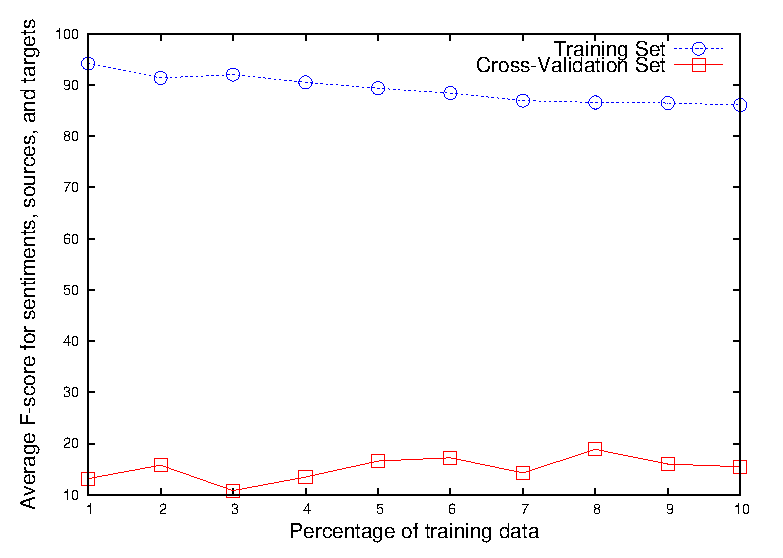
\includegraphics[width = 0.9\textwidth,height=170px]{img/lrn_curve.eps}
  \end{figure}
\end{frame}

\begin{frame}{Problems and Open Questions}
  \begin{itemize}
  \item Bad overfitting;
  \item Inconsistent tagging sequences;
  \item Flat tagging scheme;
  \item Relation linking.
  \end{itemize}
\end{frame}

\begin{frame}{Preliminary Conclusions and Perspectives}
  Conclusions:
  \begin{itemize}
  \item Preprocessing matters (w/25.067 vs. wo/18.277);
  \item Quality of polarity dictionaries is important (sentiws/25.067 vs. gpc/23.903);
  \end{itemize}

  Perspectives:
  \begin{itemize}
  \item Different classifiers (higher order CRFs, structural SVMs, etc.);
  \item Experiments with polarity dictionaries and ontologies;
  \end{itemize}
\end{frame}

\begin{frame}{}
  \begin{table}
    \tiny
    \caption{\scriptsize Classification results for automatic sentiment
      analysis (binary overlap; \alt<1>{linear chain}{tree-structured} CRFs).}
    \centering
    \begin{tabular}{p{0.25\textwidth}*{3}{>{\centering\arraybackslash}p{0.15\textwidth}}}
      \hline\noalign{\smallskip}
      Classification Element & Precision & Recall & F-Measure\\\hline
      \multicolumn{4}{c}{\cellcolor{lightcyan4}Training Set}\\
      \alt<1>{
        Sentiment & 98.73 & 95.84 & 97.26\\
        Source & 94.71 & 94.3 & 94.51\\
        Target & 97.22 & 94.87 & 96.03\\
      }{
        Sentiment & 41.68 & 73.12 & 53.1\\
        Source & 44.13 & 67.54 & 53.38\\
        Target & 29.46 & 74.67 & 42.25\\
      }
      \hline\multicolumn{4}{c}{\cellcolor{lightcyan4}Test Set}\\
      \alt<1>{
        Sentiment & 34.24 & 18.81 & 24.28\\
        Source & 27.78 & 10 & 14.71\\
        Target & 24.5 & 20.75 & 22.47\\
      }{
        Sentiment & 24.86 & 27.46 & 26.09\\
        Source & 19.78 & 18 & 18.85\\
        Target & 18.24 & 30.26 & 22.76\\
      }
      \noalign{\smallskip} \hline
    \end{tabular}
  \end{table}
  \pause
\end{frame}

\begin{frame}{}
  \begin{table}
    \tiny
    \caption{\scriptsize Classification results for automatic sentiment
      analysis (binary overlap; \alt<1>{linear chain}{tree-structured} CRFs).}
    \centering
    \begin{tabular}{p{0.25\textwidth}*{3}{>{\centering\arraybackslash}p{0.15\textwidth}}}
      \hline\noalign{\smallskip}
      Classification Element & Precision & Recall & F-Measure\\\hline
      \multicolumn{4}{c}{\cellcolor{lightcyan4}Training Set}\\
      \alt<1>{
        Sentiment & 98.22 & 97.75 & 97.98\\
        Source & 94.87 & 97.37 & 96.1\\
        Target & 97.55 & 95.88 & 96.71\\
      }{
        Sentiment & 55.82 & 77.15 & 64.78\\
        Source & 57.38 & 75 & 65.02\\
        Target & 31.2 & 73.67 & 43.83\\
      }
      \hline\multicolumn{4}{c}{\cellcolor{lightcyan4}Test Set}\\
      \alt<1>{
        Sentiment & 64.3 & 48.14 & 55.06\\
        Source & 51.72 & 30 & 37.97\\
        Target & 32.26 & 32.28 & 32.27\\
      }{
        Sentiment & 47.02 &  49.49 & 48.23\\
        Source & 29.27 & 24 & 26.37\\
        Target & 19.74 & 32.28 & 24.5\\
      }
      \noalign{\smallskip} \hline
    \end{tabular}
  \end{table}
  \pause
\end{frame}

%%%%%%%%%%%%%%%%%%%%%%%%%%%%%%%%%%%%%%%%%%%%%%%%%%%%%%%%%%%%%%%%%%
%%% Fine-grained Sentiment Analysis
\section*{Bibliography}
\bibliography{bibliography}
\bibliographystyle{plain}
\end{document}
